\chapter{Engineering Design\label{chap:design}}
% 中文版：
% 本章将对该工程的系统架构进行详细阐述，系统总架构如图Figure~\ref{fig:overall_architecture}所示。

%接下来将针对建图架构、定位架构、无人机递送架构、导航架构等部分进行分别介绍。

% English Version：
This chapter will provide a description of the system design for the engineering, including use case, architecture and data flow. Next, we will introduce them one by one.

\section{Use Case}
First of all, we will introduce the use case of the engineering. The use case is shown in Figure~\ref{fig:use_case}.
\begin{figure}[h]
    \centering
    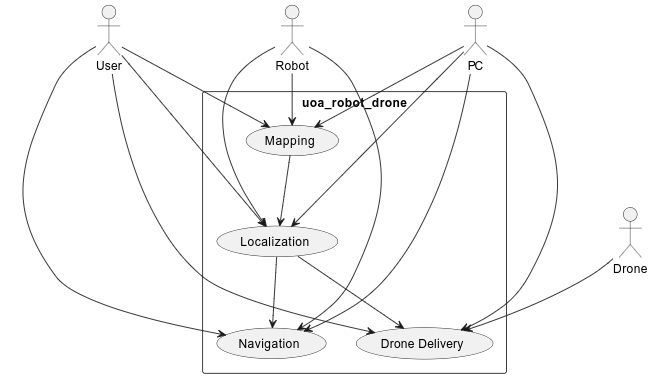
\includegraphics[width=0.9\textwidth]{figs/uml/use_case.png}
    \caption{Use Case}
    \label{fig:use_case}
\end{figure}
There are four actors in the use case:
\begin{itemize}
    \item \textbf{User}: The user can control the robot to move around, set a target position, and monitor the robot's status.
    \item \textbf{Robot}: The robot can perform mapping, localization, and navigation tasks, and can also deliver items using a drone.
    \item \textbf{Drone}: The drone can be controlled by the robot to deliver items to a specified target position.
    \item \textbf{PC}: The PC is a personal computer that runs the uoa\_robot\_drone engineering package, which includes nodes for monitoring the robot's status and controlling the drone.
\end{itemize}
There are four main use cases in the use case diagram:
\begin{itemize}
    \item \textbf{Mapping}: The robot can perform mapping tasks to create a map of the environment.
    \item \textbf{Localization}: The robot can determine its position in the environment using the map created during the mapping stage.
    \item \textbf{Drone Delivery}: The robot can control the drone to deliver items to a specified target position.
    \item \textbf{Navigation}: The robot can navigate to a specified target position using the map created during the mapping stage and the localization information. 
\end{itemize}
The following section is Engineering System Architecture.

\section{Engineering System Architecture}
This distributed system architecture consists of three main components: Raspberry Pi, Jetson Orin Nano, and Personal Computer. Each component integrates multiple hardware and software modules, as shown in Figure~\ref{fig:system_architecture}, to collaboratively accomplish mapping, localization, navigation, and drone delivery tasks.
\begin{figure}[htbp]
    \centering
    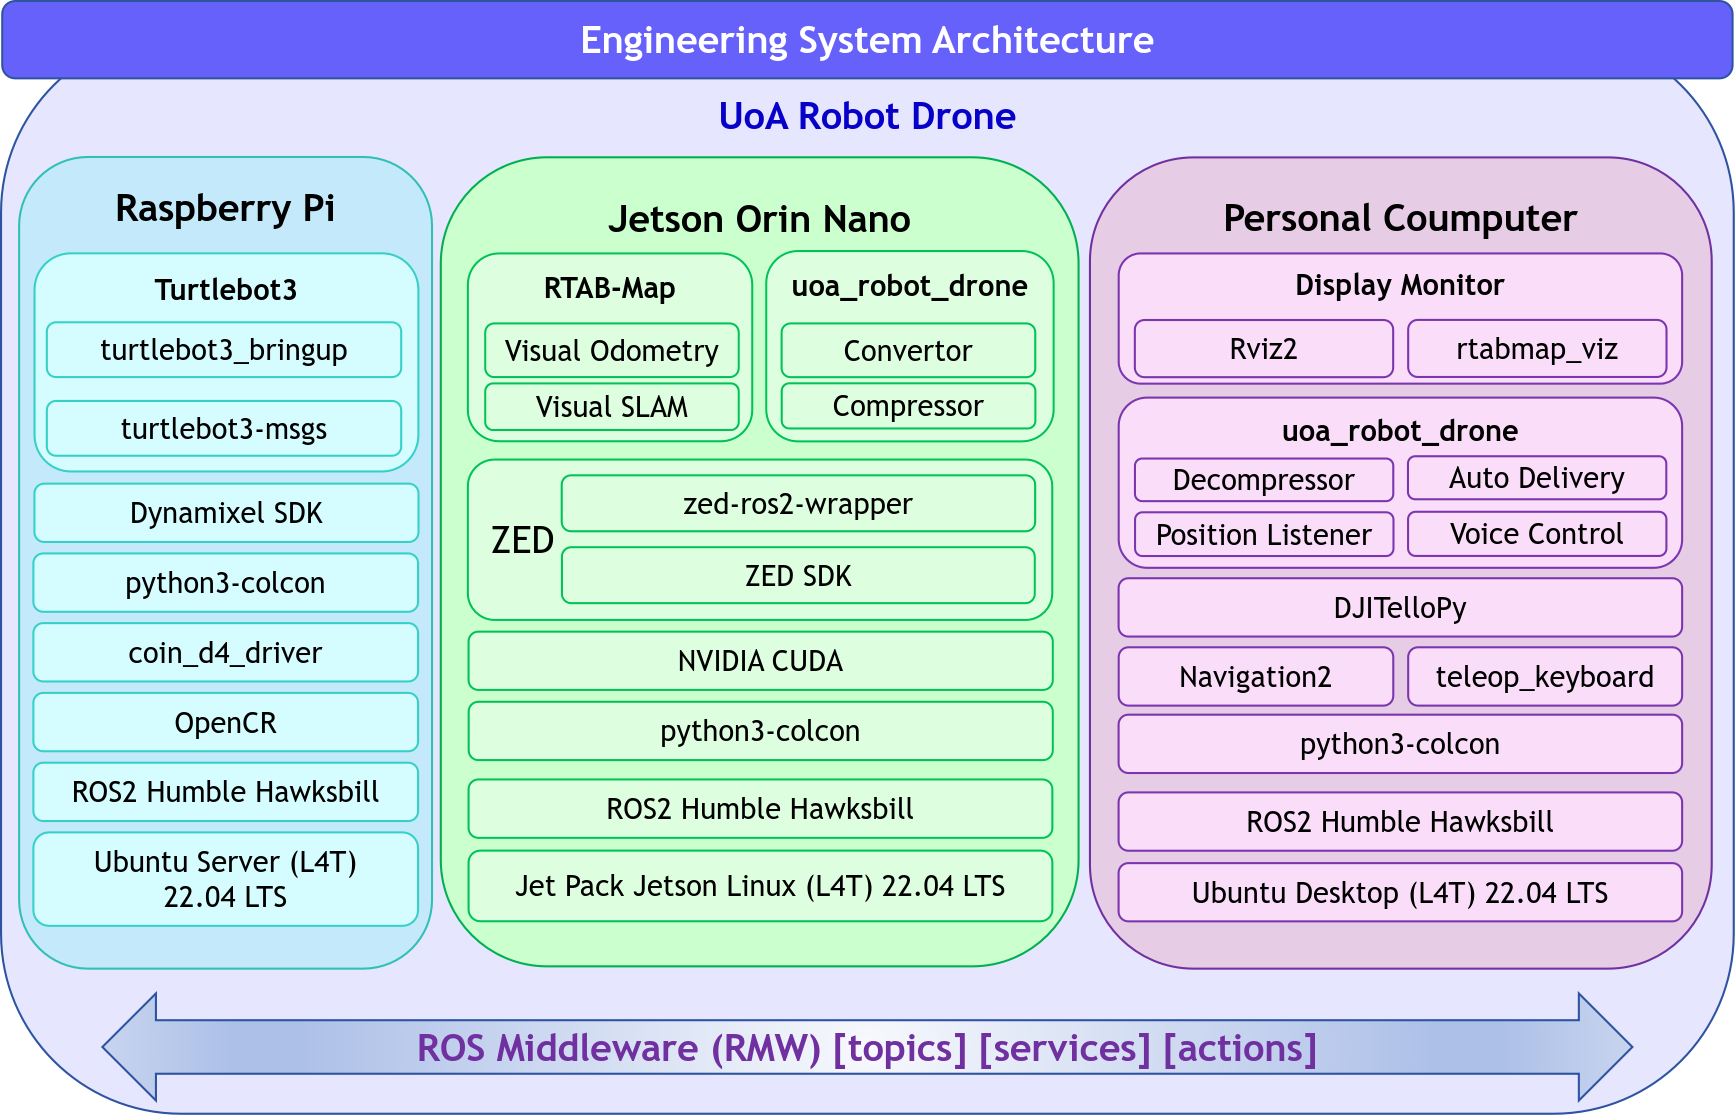
\includegraphics[width=0.9\textwidth]{figs/architecture/architecture.png}
    \caption{Engineering System Architecture}
    \label{fig:system_architecture}
\end{figure}

\begin{itemize}
    \item \textbf{Raspberry Pi}:
    \begin{itemize}
        \item \textbf{Turtlebot3}:
        \begin{itemize}
            \item \texttt{turtlebot3\_bringup}: Launches core robot nodes and drivers.
            \item \texttt{turtlebot3-msgs}: Defines message types for robot communication.
        \end{itemize}
        \item \texttt{Dynamixel SDK}: Motor control library for actuators.
        \item \texttt{python3-colcon}: ROS2 build and package management tool.
        \item \texttt{coin\_d4\_driver}: Driver for additional hardware components.
        \item \texttt{OpenCR}: Controller board for sensors and actuators.
        \item \texttt{ROS2 Humble Hawksbill}: Robot Operating System for distributed communication.
        \item \texttt{Ubuntu Server (L4T) 22.04 LTS}: Operating system for the Raspberry Pi.
    \end{itemize}

    \item \textbf{Jetson Orin Nano}:
    \begin{itemize}
        \item \textbf{RTAB-Map}:
        \begin{itemize}
            \item Visual Odometry: Estimates robot motion from camera data.
            \item Visual SLAM: Simultaneous localization and mapping.
        \end{itemize}
        \item \textbf{uoa\_robot\_drone}:
        \begin{itemize}
            \item Convertor: Image format conversion ($bgra8 \rightarrow bgr8$) for efficient processing.
            \item Compressor: Compresses image data for transmission.
        \end{itemize}
        \item \textbf{ZED}:
        \begin{itemize}
            \item \texttt{zed-ros2-wrapper}: ROS2 interface for ZED stereo camera.
            \item \texttt{ZED SDK}: Provides stereo vision and depth data.
        \end{itemize}
        \item \texttt{NVIDIA CUDA}: GPU acceleration for vision algorithms.
        \item \texttt{python3-colcon}, \texttt{ROS2 Humble Hawksbill}: As above.
        \item \texttt{Jet Pack Jetson Linux (L4T) 22.04 LTS}: Operating system for Jetson Orin Nano.
    \end{itemize}

    \item \textbf{Personal Computer}:
    \begin{itemize}
        \item \textbf{Display Monitor}:
        \begin{itemize}
            \item \texttt{Rviz2}: Visualization of robot state and environment.
            \item \texttt{rtabmap\_viz}: SLAM and mapping visualization.
        \end{itemize}
        \item \textbf{uoa\_robot\_drone}:
        \begin{itemize}
            \item Decompressor: Decompresses image data from Jetson.
            \item Auto Delivery: Controls drone delivery tasks.
            \item Position Listener: Monitors robot/drone position.
            \item Voice Control: Enables voice command interface.
        \end{itemize}
        \item \texttt{DJITelloPy}: Python library for controlling DJI Tello drone.
        \item \texttt{Navigation2}: Path planning and autonomous navigation.
        \item \texttt{teleop\_keyboard}: Manual robot control via keyboard.
        \item \texttt{python3-colcon}, \texttt{ROS2 Humble Hawksbill}: As above.
        \item \texttt{Ubuntu Desktop (L4T) 22.04 LTS}: Operating system for the PC.
    \end{itemize}
\end{itemize}

All modules communicate via ROS2 middleware (topics, services, actions), enabling seamless data exchange and coordinated operation across the distributed system.


% The next section will introduce the module sequence of each use case.

% \section{Module Sequence}
% This section will state four module sequences for the use cases of mapping, localization, drone delivery, and navigation. 
% \subsection{Mapping Module Sequence}
% The mapping module sequence is shown in Figure~\ref{fig:mapping_sequence}.
% \begin{figure}[htbp]
%     \centering
%     \includegraphics[width=0.9\textwidth]{figs/uml/mapping_sequence.png}
%     \caption{Mapping Module Sequence}
%     \label{fig:mapping_sequence}
% \end{figure}

The next section will introduce the \textbf{Data Flow} of the engineering system.

\section{Data Flow}
The data flow is shown in Figure~\ref{fig:data_flow}.

\begin{figure}[htbp]
    \centering
    
\includegraphics[width=0.9\textwidth]{figs/architecture/data_flow.png}
    \caption{Data Flow}
    \label{fig:data_flow}
\end{figure}

% 中文版：
% \begin{itemize}
% Figure~\ref{fig:data_flow}中图例解释：
%   \item 椭圆形：表示工作包或节点(teleop_keyboard,rtabmap_viz, rviz2代表节点，其它为工作包)
%   \item 嵌套圆角矩形: \\
%       * 外层表示工作包 \\
%       * 内层表示launch文件 \\
%   \item 直角矩形：\\
%       * 以"/"开头的表示ROS话题
%       * 以字母开头的表示数据
%   \item 箭头：表示数据流向，其中：
%       * 实线箭头表示一直存在的数据流向
%       * 虚线箭头表示数据流向在某些阶段才存在，如rtabmap包中的/map话题在建图阶段存在，导航阶段不存在，由navigation2包中的/map_server节点发布的/map话题在导航阶段存在，建图阶段不存在。
%   \item 圆柱形：表示数据存储
%   \item 尖圆型：表示地图数据
%   \item TF：表示坐标变换
% \end{itemize}
% 具体数据流如下：
% \subsection{立体相机获取左右摄像头图像数据}
% 摄像头获取外界图像数据后，会通过/zed/zed_node节点发布两类四个话题的图像数据：
% camera_info类话题：发布相机的内参和外参信息，包含相机的焦距、畸变系数等参数。发布的两个话题名称分别为：
% \begin{itemize}
%     \item /zed2/zed_node/left/camera_info
%     \item /zed2/zed_node/right/camera_info
% \end{itemize}
% camera类的这两个话题数据可以直接向下传递给rtabmap节点进行使用。
% image矫正后的图像类话题：发布矫正后的左右图像数据，包含图像的宽度、高度、编码格式等信息。发布的两个话题名称分别为：
% \begin{itemize}
%     \item /zed2/zed_node/left/image_rect_color
%     \item /zed2/zed_node/right/image_rect_color
% \end{itemize}
% 这俩image矫正后的图像类话题数据是bgr8a格式的，为降低网络传输数据量同时提高计算效率，会先把数据传给部署在Jetson Orin Nano上的uoa_robot_drone包中的convert_image_format节点进行预处理。
% \subsection{orin上的uoa_robot_drone包进行图像预处理}
% 部署在Jetson Orin Nano上的uoa_robot_drone包中的convert_image_format节点会订阅/zed/zed_node节点发布的两个矫正后的图像类话题以获取左右摄像头的bgra8格式的图像数据，将它们转换为bgr8格式的图像数据并发布到/uoa/left/image_rect_color和/uoa/right/image_rect_color两个话题上，供uoa_robot_drone包中的两个republish节点(orin_repub_left和orin_repub_right)和rtabmap包（具体包名为"rtabmap_sync"）中的stereo_sync节点订阅。为了降低网络传输数据量，两个republish节点会分别将订阅到的/uoa/left/image_rect_color和/uoa/right/image_rect_color两个话题的数据转换为compressed格式并发布到/uoa/cs5917/left/image_rect_color/compressed和/uoa/cs5917/right/image_rect_color/compressed两个话题上，供部署在PC上的两个监控节点(rtabmap_viz和rviz2)订阅。故，部署在Jetson Orin Nano上的uoa_robot_drone包中的节点会发布以下四个话题：
% \begin{itemize}
%     \item /uoa/orin/left/image_rect_color
%     \item /uoa/orin/right/image_rect_color
%     \item /uoa/cs5917/left/image_rect_color/compressed
%     \item /uoa/cs5917/right/image_rect_color/compressed
% \end{itemize}
% 
% \subsection{rtabmap包进行建图与定位}
% 接下来，rtabmap包中的节点会订阅以下4个话题的数据：
% \begin{itemize}
% \item /uoa/orin/left/image_rect_color
% \item /uoa/orin/right/image_rect_color
% \item /zed2/zed_node/left/camera_info
% \item /zed2/zed_node/right/camera_info
% \end{itemize} \\
% 进行计算，根据不同阶段(建图或定位)的职能发布相关话题，主要有：
% \begin{itemize}
%    \item /vo/odom
%       视觉里程计数据
%    \item /localization_pose
%       机器人当前位姿数据
%    \item /cloud_obstacles
%       障碍物点云数据
%    \item /map
%       发布建图过程中生成的地图数据。从图上可以看出，rtabmap到该话题的连接线用的是虚线，意为建图过程中发布该话题，导航过程中不发布该话题,导航过程中由/map_server节点发布/map话题的数据。
% \end{itemize}
% 其实，rtabmap包中的节点发布的话题还有很多，其它重要话题到后面的mapping stage、localization stage、navigation stage等章节中再进一步介绍。
% \subsection{PC上的uoa_robot_drone包接收图像、机器人当前位姿数即目标位姿据并发布控制指令给无人机}
% 接下来，部署在PC上的uoa_robot_drone包中的节点会订阅以下话题数据：
% \begin{itemize}
%     \item /uoa/cs5917/left/image_rect_color/compressed
%     \item /uoa/cs5917/right/image_rect_color/compressed
%     \item /localization_pose
%     \item /goal_pose
% \end{itemize}
% 然后会做如下工作：
% \begin{itemize}
%   \item 解压缩/uoa/cs5917/left/image_rect_color/compressed和/uoa/cs5917/right/image_rect_color/compressed两个话题的数据，得到左右摄像头的bgr8格式的图像数据。
%   \item 发布左右摄像头bgr8格式的图像数据到以下话题：
%     \begin{itemize}
%         \item /uoa/cs5917/left/image_rect_color
%         \item /uoa/cs5917/right/image_rect_color
%     \end{itemize}
%   \item 当处于无人机递送阶段时，根据从/localization_pose话题获取的机器人当前位姿数据和/goal_pose话题获取的目标位姿数据，计算出距离目标位置的距离和角度，当连续三次计算出的距离小于0.1米且角度小于0.1弧度时，向/uoa/auto_delivery话题发布delivery_signal=true的控制指令，表示无人机可以开始递送任务了。
% \end{itemize}
% \subsection{rtabmap_viz节点显示回环检测和Odometry图像数据}
% rtabmap_viz节点会订阅以下话题数据：
% \begin{itemize}
%     \item /uoa/cs5917/left/image_rect_color
%     \item /uoa/cs5917/right/image_rect_color
%     \item /zed/zed_node/left/camera_info
%     \item /zed/zed_node/right/camera_info
% \end{itemize}
% 然后将Odometry和loop closure 的图像数据显示到屏幕上。
% \subsection{rviz2节点显示地图点云数据和机器人位姿}
% rviz2节点会订阅以下话题数据：
% \begin{itemize}
%     \item /map
%      通过该话题接收地图数据
%     \item /uoa/cs5917/left/image_rect_color
%        通过该话题接收左侧摄像头的图像数据
%     \item /uoa/cs5917/right/image_rect_color
%        通过该话题接收右侧摄像头的图像数据
% \end{itemize}
% 然后将地图数据和机器人当前视野中看到的视频数据显示到屏幕上。在rviz2的地图中，点击“2D Goal Pose"按钮后，将鼠标移动到地图上，点击鼠标左键即可设置目标点，rviz2会将该目标点的位姿数据发布到/goal_pose话题上，供uoa_robot_drone和navigation2包中的相关节点订阅，以完成后续的无人机递送人物和导航任务。
% \subsection{navigation2包进行导航}
% navigation2包中的节点会订阅以下话题数据：
% \begin{itemize}
%   \item /goal_pose
%        目标位姿数据
%   \item /vo/odom
%        视觉里程计数据
%   \item /cloud_obstacles
%        障碍物点云数据
%   \item map
%        来自数据库的地图数据
% \end{itemize}
% 然后会做如下工作：
% \begin{itemize}
%   \item 根据/goal_pose话题获取的目标位姿数据、/vo/odom话题获取的视觉里程计数据和map数据，规划出机器人当前的位姿到目标位姿的全局路径和视野内路径。
%   \item 根据视野内路径和全局路径规划出机器人要执行的动作序列。
%   \item 将动作序列发布至/tb3/cmd_vel话题上，供Turtlebot3 Waffle Pi机器人订阅并执行动作序列前往目标位置。
%   \item 当机器人在视野内发现障碍物点云话题发布的障碍物阻碍前进路径时，会重新规划路径，避开障碍物。
% \end{itemize}
% \subsection{teleop_keyboard节点手动控制机器人}
% 在建图、定位、无人机递送阶段，可以使用键盘通过teleop_keyboard节点向/tb3/cmd_vel话题发布控制指令，手动控制Turtlebot3 Waffle Pi机器人前进、后退、左转、右转等动作。
% English Version:

Figure~\ref{fig:data_flow} Legend explanation: 
\begin{itemize}
    \item Ellipse: represents work packages or nodes (teleop\_keyboard, rtabmap\_viz, rviz2 represent nodes, others are work packages)
    \item Nested rounded Rectangle: 
        \begin{itemize}
            \item Outer layer represents work package (e.g., uoa\_robot\_drone)
            \item Inner layer represents the device that the package is deployed
        \end{itemize}
    \item Rectangular shape:
        \begin{itemize}
            \item Topics starting with "/" represent ROS topics
            \item Topics starting with letters represent data
        \end{itemize}
    \item Arrow: Indicates data flow direction, where:
        \begin{itemize}
            \item Solid arrow indicates a continuous data flow
            \item Dashed arrow indicates a data flow that exists only in certain stages, such as the /map topic in the rtabmap package existing during the mapping stage but not during navigation, while the /map topic published by the navigation2 package's map\_server node exists during navigation but not during mapping.
        \end{itemize}
    \item Cylinder: Represents data storage
    \item Rounded triangle: Represents map data
    \item TF: Represents coordinate transformation, which is used to transform the coordinate system of the data and more details seen section~\ref{sec:ros2_transform}.
\end{itemize} 

Next, we will introduce the data flow in detail.
\subsection{Stereo Camera Captures Left and Right Camera Image Data}

After the camera captures external image data, it publishes two types ("Camera Info" and "Image") of four topics of image data through the \texttt{/zed/zed\_node} node:
\begin{itemize}
    \item \textbf{Camera Info topics:} Publishes camera intrinsic and extrinsic parameters, including focal length, distortion coefficients, etc. The two published topic names are:
    \begin{itemize}
        \item /zed/zed\_node/left/camera\_info
        \item /zed/zed\_node/right/camera\_info 
    \end{itemize}
    The camera\_info topics can be directly passed down to the rtabmap node for use.
    \item \textbf{Image topics:} Publishes rectified left and right image data, including information such as image width, height, and encoding format. The two published topic names are:
    \begin{itemize}
        \item /zed/zed\_node/left/image\_rect\_color
        \item /zed/zed\_node/right/image\_rect\_color
    \end{itemize}
\end{itemize}

\sloppy
The two rectified image topics are in bgra8 format. To reduce network transmission data volume and improve computational efficiency, the data is first preprocessed by the \texttt{convert\_image\_format} node in the \texttt{uoa\_robot\_drone} package deployed on the Jetson Orin Nano.

\subsection{Image Preprocessing in \texttt{uoa\_robot\_drone} Package on Orin}
\sloppy
The \texttt{convert\_image\_format} node in the \texttt{uoa\_robot\_drone} package deployed on the Jetson Orin Nano subscribes to the two rectified image topics published by the \texttt{/zed/zed\_node} node to obtain the left and right camera bgra8 format image data, converts them to bgr8 format, and publishes them to the \texttt{/uoa/left/image\_rect\_color} and \texttt{/uoa/right/image\_rect\_color} topics. These topics are then subscribed to by two republish nodes (\texttt{orin\_repub\_left} and \texttt{orin\_repub\_right}) in the \texttt{uoa\_robot\_drone} package and the \texttt{stereo\_sync} node in the \texttt{rtabmap} package (specifically named \texttt{rtabmap\_sync}). To reduce network transmission data volume, the two republish nodes compress the subscribed data from \texttt{/uoa/left/image\_rect\_color} and \texttt{/uoa/right/image\_rect\_color} into compressed format and publish them to \texttt{/uoa/cs5917/left/image\_rect\_color/compressed} and \texttt{/uoa/cs5917/right/image\_rect\_color/compressed} topics, which are then subscribed to by two uncompressed nodes (\texttt{uoa\_pc\_repub\_left} and \texttt{uoa\_pc\_repub\_right}) and uncompressed and finally are used by monitoring nodes (\texttt{rtabmap\_viz} and \texttt{rviz2}) deployed on the PC. Therefore, the nodes in the \texttt{uoa\_robot\_drone} package deployed on the Jetson Orin Nano will publish the following four topics:
\begin{itemize}
    \item \texttt{/uoa/orin/left/image\_rect\_color}
    \item \texttt{/uoa/orin/right/image\_rect\_color}
    \item \texttt{/uoa/cs5917/left/image\_rect\_color/compressed}
    \item \texttt{/uoa/cs5917/right/image\_rect\_color/compressed}
\end{itemize}

\subsection{rtabmap Package for Mapping and Localization}
Next, the nodes in the rtabmap package will subscribe to the data from the following four topics:
\begin{itemize}
    \item \texttt{/uoa/orin/left/image\_rect\_color}
    \item \texttt{/uoa/orin/right/image\_rect\_color}
    \item \texttt{/zed/zed\_node/left/camera\_info}
    \item \texttt{/zed/zed\_node/right/camera\_info}
\end{itemize}
to perform calculations and publish relevant topics based on different stages (mapping or localization), mainly including:
\begin{itemize}
    \item \texttt{/vo/odom} \\
        Visual odometry data
    \item \texttt{/localization\_pose} \\
        Current robot pose data
    \item \texttt{/cloud\_obstacles} \\
        Obstacle point cloud data
    \item \texttt{/map} \\
        Publishes the map data generated during the mapping process. As shown in the figure, the connection line to this topic from \texttt{rtabmap} is a dashed line, indicating that this topic is published during the mapping stage but not during navigation. During navigation, the \texttt{/map} topic is published by the \texttt{map\_server} node in the \texttt{navigation2} package.
\end{itemize}
In fact, here we only introduce some important topics published by the nodes in the rtabmap package. Other topics can be found in Appendix~\ref{app:ros2graphs}.

\subsection{\texttt{uoa\_robot\_drone} Package on PC Receives Image, Robot Current Pose, and Target Pose Data, and Publishes Control Commands to Drone}
Next, the nodes in the \texttt{uoa\_robot\_drone} package deployed on the PC will subscribe to the data from the following topics:
\begin{itemize}
    \item \texttt{/uoa/cs5917/left/image\_rect\_color/compressed}
    \item \texttt{/uoa/cs5917/right/image\_rect\_color/compressed}
    \item \texttt{/localization\_pose}
    \item \texttt{/goal\_pose}
\end{itemize}
Then, it will perform the following tasks:
\begin{itemize}
    \item Decompress the data from \texttt{/uoa/cs5917/left/image\_rect\_color/compressed} and \texttt{/uoa/cs5917/right/image\_rect\_color/compressed} topics to obtain the left and right camera bgr8 format image data.
    \item Publish the left and right camera bgr8 format image data to the following topics:
    \begin{itemize}
    \item \texttt{/uoa/cs5917/left/image\_rect\_color}
    \item \texttt{/uoa/cs5917/right/image\_rect\_color}
    \end{itemize}
    \item When in the drone delivery stage, calculate the distance and angle to the target position based on the current robot pose data obtained from the \texttt{/localization\_pose} topic and the target pose data obtained from the \texttt{/goal\_pose} topic. If the distance is less than 0.1 meters and the angle is less than 0.1 radians for three consecutive calculations, a control command with delivery\_signal=true is published to the \texttt{/uoa/auto\_delivery} topic, indicating that the drone can start the delivery task.
\end{itemize}

\subsection{\texttt{rtabmap\_viz} Node Displays Loop Closure Detection and Odometry Image Data}
The \texttt{rtabmap\_viz} node will subscribe to the data from the following topics:
\begin{itemize}
    \item \texttt{/uoa/cs5917/left/image\_rect\_color}
    \item \texttt{/uoa/cs5917/right/image\_rect\_color}
    \item \texttt{/zed/zed\_node/left/camera\_info}
    \item \texttt{/zed/zed\_node/right/camera\_info}
\end{itemize}
Then, it will display the Odometry and loop closure images on the screen.
\subsection{rviz2 Node Displays Map Point Cloud Data and Robot Pose}
The \texttt{rviz2} node will subscribe to the data from the following topics:
\begin{itemize}
     \item \texttt{/map}
        Receives map data through this topic
     \item \texttt{/uoa/cs5917/left/image\_rect\_color}
         Receives left camera image data through this topic
     \item \texttt{/uoa/cs5917/right/image\_rect\_color}
         Receives right camera image data through this topic
\end{itemize}
Then, it will display the map data and the video data seen by the robot in its current field of view on the screen. In \texttt{rviz2}'s map, after clicking the "2D Goal Pose" button, move the mouse to the map and click the left mouse button to set the target point. \texttt{rviz2} will publish the pose data of this target point to the \texttt{/goal\_pose} topic, which will be subscribed to by the \texttt{uoa\_robot\_drone} and related nodes in the \texttt{navigation2} package to complete subsequent drone delivery tasks and navigation tasks.
\subsection{\texttt{navigation2} Package for Navigation}
The nodes in the \texttt{navigation2} package will subscribe to the data from the following topics:
\begin{itemize}
     \item \texttt{/goal\_pose}
         Target pose data
     \item \texttt{/vo/odom}
         Visual odometry data
     \item \texttt{/cloud\_obstacles}
         Obstacle point cloud data
  \item \texttt{map}
         Map data from the database
\end{itemize}
Then, it will perform the following tasks:
\begin{itemize}
    \item Based on the target pose data obtained from the \texttt{/goal\_pose} topic, the visual odometry data obtained from the \texttt{/vo/odom} topic, and the map data, it will plan the global path from the robot's current pose to the target pose and the path within the field of view.
    \item Plan the action sequence for the robot to execute based on the path within the field of view and the global path.
        \item Publish the action sequence to the \texttt{/tb3/cmd\_vel} topic for the \texttt{Robot} to subscribe and execute the action sequence to move towards the target position.
        \item When the robot detects obstacles in its path through the obstacle point cloud data published on the \texttt{/cloud\_obstacles} topic, it will replan the path to avoid the obstacles.
\end{itemize}

\subsection{\texttt{teleop\_keyboard} Node for Manual Robot Control}
During the mapping, localization, and drone delivery stages, user can manually control the \texttt{Robot} to move forward, backward, turn left, and turn right by publishing control commands to the \texttt{/tb3/cmd\_vel} topic using the keyboard through the \texttt{teleop\_keyboard} node.
